\section{Results}

\begin{frame}{}
    \tableofcontents[currentsection]
\end{frame}



% \subsection{Test Case 1: 6-bus Grid}

% \begin{frame}{Case 6-bus Grid (1)}
%     \begin{figure}[H]
%         \centering
%         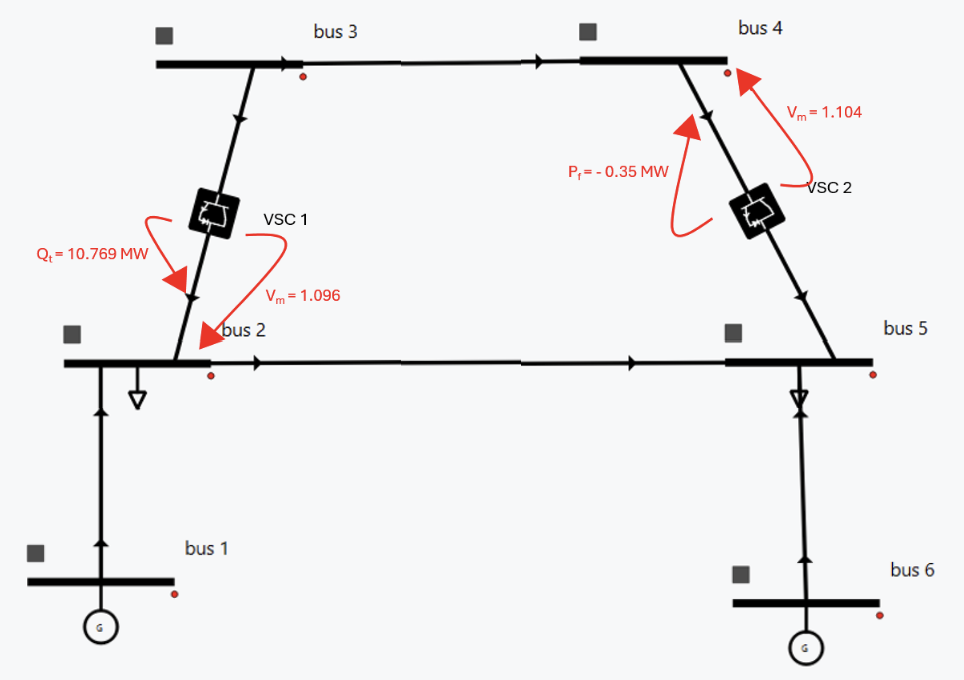
\includegraphics[width=0.7\textwidth]{chapter5pics/busSmall.png}
%         \caption{6-bus system including two VSCs.}
%         \label{fig:simple6bus}
%     \end{figure}
% \end{frame}



% \begin{frame}{Case 6-bus Grid (3)}

%     \begin{figure}[H]
%         \centering
%         \begin{minipage}{0.5\textwidth}
%             \centering
%             % Raw Error Evolution Plot
%             \begin{tikzpicture}
%             \begin{semilogyaxis}[
%                 title={\textbf{Raw Error Evolution}},
%                 xlabel={Iterations},
%                 ylabel={log(Error) (p.u.)},
%                 width=\textwidth,
%                 height=0.8\textwidth,  % Increased height
%                 xmin=1, xmax=7,
%                 ymin=1e-8, ymax=1e1,
%                 log base 10 number format code/.code={\pgfmathprintnumber[fixed]{####1}},
%                 max space between ticks=20,
%                 legend pos=north east,
%                 ymajorgrids=true,
%                 grid style=dashed,
%                 scaled ticks=false,
%                 yticklabel style={/pgf/number format/sci},
%                 legend style={font=\footnotesize},
%             ]
        
%             % Data for 'Generalised Raw Error'
%             \addplot[
%                 color=blue,
%                 mark=*,
%                 mark options={solid}
%                 ]
%                 coordinates {
%                     (1, 2.6892240045602778)
%                     (2, 0.394526169257302)
%                     (3, 0.05930097210068633)
%                     (4, 0.0008398038807334203)
%                     (5, 1.8931955975826087e-07)
%                     (6, 0)
%                     (7, 0)
%                 };
%                 \addlegendentry{Generalised}
        
%             % Data for 'Classical Raw Error'
%             \addplot[
%                 color=orange,
%                 mark=square*,
%                 mark options={solid}
%                 ]
%                 coordinates {
%                     (1, 1.269404698187123)
%                     (2, 0.18109495944614842)
%                     (3, 0.06623071061244291)
%                     (4, 0.0010452365749415889)
%                     (5, 0.0008880971365704372)
%                     (6, 5.708852986144179e-05)
%                     (7, 2.1547763279882262e-07)
%                 };
%                 \addlegendentry{Classical}
%             \end{semilogyaxis}
%             \end{tikzpicture}
%         \end{minipage}\hfill
%         \begin{minipage}{0.5\textwidth}
%             \centering
%             % Normalized Error Evolution Plot
%             \begin{tikzpicture}
%             \begin{semilogyaxis}[
%                 title={\textbf{Normalized Error Evolution}},
%                 xlabel={Iterations},
%                 ylabel={log(Error) (p.u.)},
%                 width=\textwidth,
%                 height=0.8\textwidth,  % Increased height
%                 xmin=1, xmax=7,
%                 ymin=1e-8, ymax=1e1,
%                 log base 10 number format code/.code={\pgfmathprintnumber[fixed]{####1}},
%                 max space between ticks=20,
%                 legend pos=south west,
%                 ymajorgrids=true,
%                 grid style=dashed,
%                 scaled ticks=false,
%                 yticklabel style={/pgf/number format/sci},
%                 legend style={font=\footnotesize},
%             ]
        
%             % Data for 'Generalised Normalized Error'
%             \addplot[
%                 color=blue,
%                 mark=*,
%                 mark options={solid}
%                 ]
%                 coordinates {
%                     (1, 1.0)
%                     (2, 1.46706324e-01)
%                     (3, 2.20513323e-02)
%                     (4, 3.12284837e-04)
%                     (5, 7.03993269e-08)
%                     (6, 0)
%                     (7, 0)
%                 };
%                 \addlegendentry{Generalised}
        
%             % Data for 'Classical Normalized Error'
%             \addplot[
%                 color=orange,
%                 mark=square*,
%                 mark options={solid}
%                 ]
%                 coordinates {
%                     (1, 1.00)
%                     (2, 1.42661328e-01)
%                     (3, 5.21746223e-02)
%                     (4, 8.23406890e-04)
%                     (5, 6.99617024e-04)
%                     (6, 4.49726789e-05)
%                     (7, 1.69746995e-07)
%                 };
%                 \addlegendentry{Classical}
%             \end{semilogyaxis}
%             \end{tikzpicture}
%         \end{minipage}
%     \end{figure}
%     \caption{Error evolution for 6-bus system: Raw and Normalized.}
% \end{frame}

% \begin{frame}{Case 6-bus Grid (4)}

%     \begin{figure}[H]
%         \begin{minipage}{0.5\textwidth}
%             \centering
%             % Voltage Magnitudes Plot
%             \begin{tikzpicture}
%             \begin{axis}[
%                 title={\textbf{Voltage Magnitudes $\mathcal{V}$}},
%                 xlabel={Bus},
%                 ylabel={$\mathcal{V}$ (p.u.)},
%                 width=0.9\textwidth,
%                 xmin=1, xmax=6,
%                 ymin=1.0, ymax=1.2,
%                 xtick={1,2,3,4,5,6},
%                 ytick={1.0, 1.05, 1.10, 1.15, 1.2},
%                 legend pos=north east,
%                 legend style = {font = \tiny},
%                 ymajorgrids=true,
%                 grid style=dashed,
%             ]
    
%             % Voltage Magnitudes for Generalised
%             \addplot[
%                 color=blue,
%                 mark=square,
%                 ]
%                 coordinates {
%                     (1, 1.100000) 
%                     (2, 1.096000) 
%                     (3, 1.097501) 
%                     (4, 1.104000) 
%                     (5, 1.111759) 
%                     (6, 1.120000)
%                 };
%                 \addlegendentry{Generalised}
    
%             % Voltage Magnitudes for Classical
%             \addplot[
%                 color=red,
%                 mark=o,
%                 ]
%                 coordinates {
%                     (1, 1.100000) 
%                     (2, 1.096000) 
%                     (3, 1.0975009057971015) 
%                     (4, 1.1040000000000003) 
%                     (5, 1.1118905176618838) 
%                     (6, 1.1200000000000003)
%                 };
%                 \addlegendentry{Classical}
    
%             \end{axis}
%             \end{tikzpicture}
%         \end{minipage}\hfill
%         \begin{minipage}{0.5\textwidth}
%             \centering
%             % Voltage Angles Plot
%             \begin{tikzpicture}
%             \begin{axis}[
%                 title={\textbf{Voltage Angles $\theta$}},
%                 xlabel={Bus},
%                 ylabel={$\theta$ (º)},
%                 width = 0.9\textwidth,
%                 xmin=1, xmax=6,
%                 ymin=-5, ymax=5,
%                 xtick={1,2,3,4,5,6},
%                 ytick={-5, 0, 5},
%                 legend pos=south west,
%                 legend style = {font = \tiny},
%                 ymajorgrids=true,
%                 grid style=dashed,
%             ]
    
%             % Voltage Angles for Generalised
%             \addplot[
%                 color=blue,
%                 mark=square,
%                 ]
%                 coordinates {
%                     (1, 0.000) 
%                     (2, -0.2616) 
%                     (3, 0.000) 
%                     (4, 0.000) 
%                     (5, -4.023) 
%                     (6, -3.981)
%                 };
%                 \addlegendentry{Generalised}
    
%             % Voltage Angles for Classical
%             \addplot[
%                 color=red,
%                 mark=o,
%                 ]
%                 coordinates {
%                     (1, 0.000) 
%                     (2, -0.2617489390790084) 
%                     (3, 4.386384618139598) 
%                     (4, 4.386384618139602) 
%                     (5, -4.023100366977882) 
%                     (6, -3.9812657581331665)
%                 };
%                 \addlegendentry{Classical}
    
%             \end{axis}
%             \end{tikzpicture}
%         \end{minipage}
%         \caption{Voltage comparison for the Case 6-bus system: Generalised vs Classical.}
%         \label{fig:v_6bus}
%     \end{figure}

% \end{frame}



% \begin{frame}{Case 6-bus Grid (5)}

%     % Table for VSC 1 Branch Powers
%     \begin{table}[H]
%         \centering
%         \caption{Comparison of VSC 1 branch powers.}
%         \begin{tabular}{lcc}
%         \hline
%         \textbf{Power Flow} & \textbf{Generalised (MW/Mvar)} & \textbf{Classical (MW/Mvar)} \\ \hline\hline
%         Pf (Active Power From)  & 0.3479  & 0.3479 \\ 
%         Qf (Reactive Power From) & 0       & 0 \\ 
%         Pt (Active Power To)     & 0.7437  & 0.7437 \\ 
%         Qt (Reactive Power To)   & 10.77   & 10.77  \\ \hline
%         \end{tabular}
        
%         \label{tab:vsc1Comparison}
%     \end{table}

%     % Table for VSC 2 Branch Powers
%     \begin{table}[H]
%         \centering
%         \caption{Comparison of VSC 2 branch powers.}
%         \begin{tabular}{lcc}
%         \hline
%         \textbf{Power Flow} & \textbf{Generalised (MW/Mvar)} & \textbf{Classical (MW/Mvar)} \\ \hline\hline
%         Pf (Active Power From)  & -0.3500 & -0.3500 \\ 
%         Qf (Reactive Power From) & 0   & 0 \\ 
%         Pt (Active Power To)     & 0.3794 & 0.3793 \\ 
%         Qt (Reactive Power To)   & 1.550  & 1.550  \\ \hline
%         \end{tabular}
        
%         \label{tab:vsc2Comparison}
%     \end{table}

% \end{frame}



   

% \subsection{Test Case 2: Modified IEEE 14-bus}

% \begin{frame}{Modified IEEE 14-bus (1)}

% \begin{figure}[H]
%     \centering
%     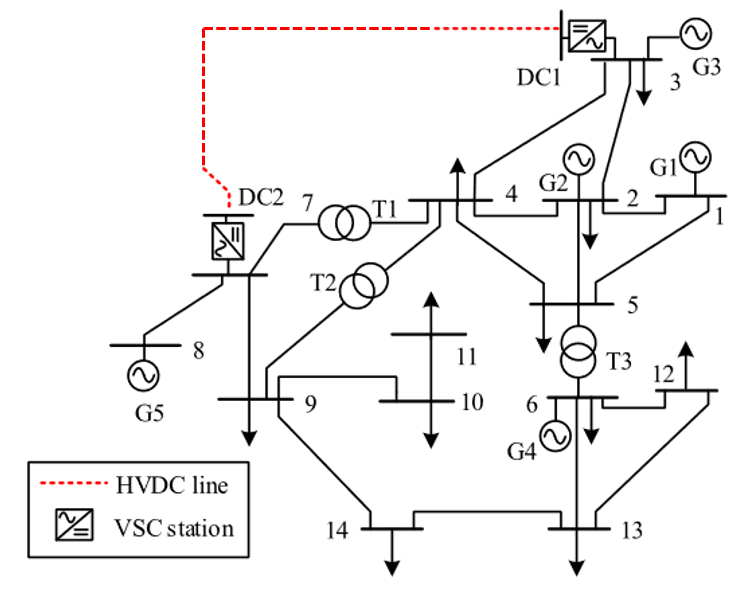
\includegraphics[width=0.6\textwidth]{chapter5pics/modifiedIEEEexample.png}
%     \caption{Modified IEEE 14-bus System.}
%     \label{fig:modifiedIEEE14Bus}
% \end{figure}
% \end{frame}


% % \begin{frame}{Modified IEEE 14-bus (2)}

% % \begin{figure}[H]
% %     \centering
% %     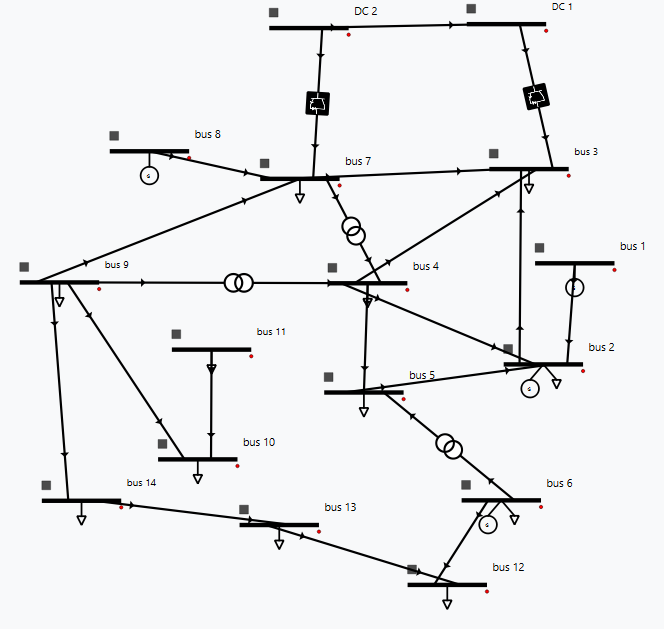
\includegraphics[width=0.6\textwidth]{chapter5pics/IEEE14gridcal.png}
% %     \caption{Modified IEEE 14-bus system in GridCal.}
% %     \label{fig:14busACDCGrdical}
% % \end{figure}
% % \end{frame}


% \begin{frame}{Modified IEEE 14-bus (2)}
% \begin{figure}[H]
%     \centering
%     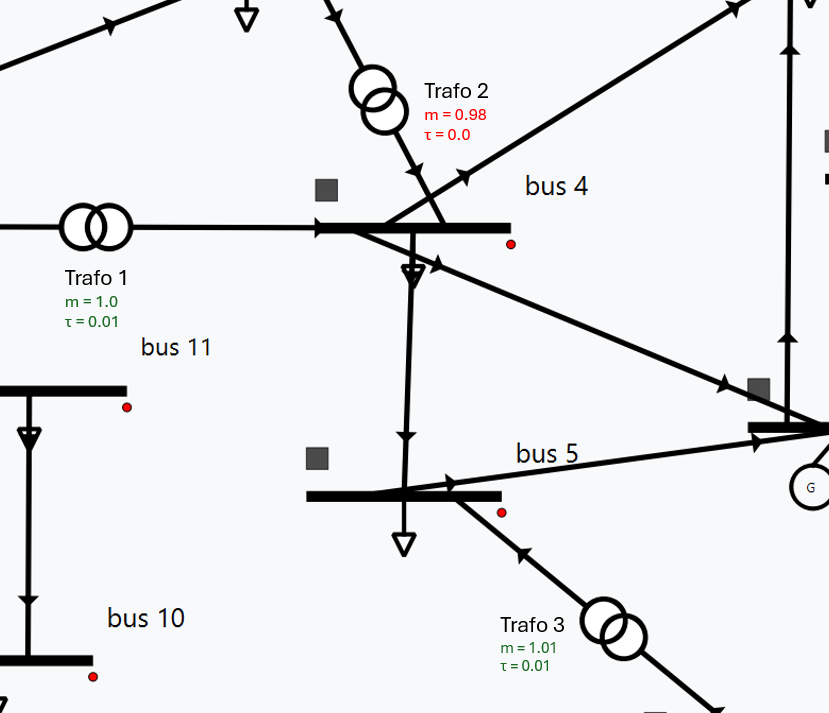
\includegraphics[width=0.6\textwidth]{chapter5pics/controlModeswithWords.png}
%     \caption{Control Mode for Controllable Transformer Trafo 2.}
%     \label{fig:vscControls}
% \end{figure}
% \end{frame}


% \begin{frame}{Modified IEEE 14-bus (3)}

%     \begin{figure}[H]
%         \centering
%         \begin{minipage}{0.5\textwidth}
%             \centering
%             % Raw Error Evolution Plot
%             \begin{tikzpicture}
%             \begin{semilogyaxis}[
%                 title={\textbf{Raw Error Evolution}},
%                 xlabel={Iterations},
%                 ylabel={log(Error) (p.u.)},
%                 width=\textwidth,
%                 height=0.8\textwidth,  % Increased height
%                 xmin=1, xmax=10,
%                 ymin=1e-9, ymax=1e2,
%                 log base 10 number format code/.code={\pgfmathprintnumber[fixed]{####1}},
%                 max space between ticks=20,
%                 legend pos=north east,
%                 ymajorgrids=true,
%                 grid style=dashed,
%                 scaled ticks=false,
%                 yticklabel style={/pgf/number format/sci},
%                 legend style={font=\footnotesize},
%             ]
        
%             % Data for 'Generalised Raw Error'
%             \addplot[
%                 color=blue,
%                 mark=*,
%                 mark options={solid}
%                 ]
%                 coordinates {
%                     (1, 11.540345759133386)
%                     (2, 9.326041440251467)
%                     (3, 3.4197248835090437)
%                     (4, 0.060678315324364344)
%                     (5, 9.099329239091458e-05)
%                     (6, 4.331210120454077e-07)
%                     (7, 3.9953538837903874e-09)
%                     (8, 3.843241811167149e-11)
%                     (9, 0)
%                     (10, 0)
%                 };
%                 \addlegendentry{Generalised}
        
%             % Data for 'Classical Raw Error'
%             \addplot[
%                 color=orange,
%                 mark=square*,
%                 mark options={solid}
%                 ]
%                 coordinates {
%                     (1, 13.5)
%                     (2, 10.0)
%                     (3, 5.5)
%                     (4, 1.2)
%                     (5, 0.05)
%                     (6, 0.0005)
%                     (7, 2.5e-05)
%                     (8, 1e-07)
%                     (9, 1e-09)
%                     (10, 0)
%                 };
%                 \addlegendentry{Classical}
%             \end{semilogyaxis}
%             \end{tikzpicture}
%         \end{minipage}\hfill
%         \begin{minipage}{0.5\textwidth}
%             \centering
%             % Normalized Error Evolution Plot
%             \begin{tikzpicture}
%             \begin{semilogyaxis}[
%                 title={\textbf{Normalized Error Evolution}},
%                 xlabel={Iterations},
%                 ylabel={log(Error) (p.u.)},
%                 width=\textwidth,
%                 height=0.8\textwidth,  % Increased height
%                 xmin=1, xmax=10,
%                 ymin=1e-9, ymax=1e2,
%                 log base 10 number format code/.code={\pgfmathprintnumber[fixed]{####1}},
%                 max space between ticks=20,
%                 legend pos=north east,
%                 ymajorgrids=true,
%                 grid style=dashed,
%                 scaled ticks=false,
%                 yticklabel style={/pgf/number format/sci},
%                 legend style={font=\footnotesize},
%             ]
        
%             % Data for 'Generalised Normalized Error'
%             \addplot[
%                 color=blue,
%                 mark=*,
%                 mark options={solid}
%                 ]
%                 coordinates {
%                     (1, 1.00000000e+00)
%                     (2, 8.08124959e-01)
%                     (3, 2.96327767e-01)
%                     (4, 5.25792871e-03)
%                     (5, 7.88479776e-06)
%                     (6, 3.75310256e-08)
%                     (7, 3.46207468e-10)
%                     (8, 3.33026574e-12)
%                     (9, 0.00000000e+00)
%                     (10, 0.00000000e+00)
%                 };
%                 \addlegendentry{Generalised}
        
%             % Data for 'Classical Normalized Error'
%             \addplot[
%                 color=orange,
%                 mark=square*,
%                 mark options={solid}
%                 ]
%                 coordinates {
%                     (1, 1.00000000e+00)
%                     (2, 7.40740741e-01)
%                     (3, 4.07407407e-01)
%                     (4, 8.88888889e-02)
%                     (5, 3.70370370e-03)
%                     (6, 3.70370370e-05)
%                     (7, 1.85185185e-06)
%                     (8, 7.40740741e-09)
%                     (9, 7.40740741e-11)
%                     (10, 0.00000000e+00)
%                 };
%                 \addlegendentry{Classical}
%             \end{semilogyaxis}
%             \end{tikzpicture}
%         \end{minipage}
%         \caption{Error evolution for Modified IEEE 14-bus system: Raw and Normalized.}
%     \end{figure}
    
% \end{frame}

% \begin{frame}{Modified IEEE 14-bus (4)}

%     \begin{figure}[H]
%         \begin{minipage}{0.5\textwidth}
%             \centering
%             % Voltage Magnitudes Plot
%             \begin{tikzpicture}
%             \begin{axis}[
%                 title={\textbf{Voltage Magnitudes $\mathcal{V}$}},
%                 xlabel={Bus},
%                 ylabel={$\mathcal{V}$ (p.u.)},
%                 width=\textwidth,
%                 height=0.8\textwidth,
%                 xmin=1, xmax=16,
%                 ymin=1.0, ymax=1.12,
%                 xtick={2,4,6,8,10,12,14,16},
%                 ytick={1.0, 1.02, 1.04, 1.06, 1.08, 1.10, 1.12},
%                 legend pos=north east,
%                 ymajorgrids=true,
%                 grid style=dashed,
%             ]
    
%             % Voltage Magnitudes for Generalised
%             \addplot[
%                 color=blue,
%                 mark=square,
%                 ]
%                 coordinates {
%                     (1, 1.0000000000000002)
%                     (2, 1.052137949683555)
%                     (3, 1.0745035368060132)
%                     (4, 1.0876337549205068)
%                     (5, 1.046047571764098)
%                     (6, 1.0000000000000002)
%                     (7, 1.096)
%                     (8, 1.1)
%                     (9, 1.0757605643463326)
%                     (10, 1.076565729465785)
%                     (11, 1.0754571130877324)
%                     (12, 1.0183332090105)
%                     (13, 1.0379486191812881)
%                     (14, 1.0548073646596836)
%                     (15, 1.104)
%                     (16, 1.0975009057971012)
%                 };
    
%             % Voltage Magnitudes for Classical
%             \addplot[
%                 color=red,
%                 mark=o,
%                 ]
%                 coordinates {
%                     (1, 1.0000000000000002)
%                     (2, 1.052137949683555)
%                     (3, 1.0745035368060132)
%                     (4, 1.086110725064099)
%                     (5, 1.046047571764098)
%                     (6, 1.0000000000000002)
%                     (7, 1.096)
%                     (8, 1.1)
%                     (9, 1.0762300387322676)
%                     (10, 1.076023169422199)
%                     (11, 1.0759205307805448)
%                     (12, 1.0187989387640701)
%                     (13, 1.037706656909722)
%                     (14, 1.0567206449043414)
%                     (15, 1.104)
%                     (16, 1.0975009057971012)
%                 };
    
%             \end{axis}
%             \end{tikzpicture}
%         \end{minipage}\hfill
%         \begin{minipage}{0.5\textwidth}
%             \centering
%             % Voltage Angles Plot
%             \begin{tikzpicture}
%             \begin{axis}[
%                 title={\textbf{Voltage Angles $\theta$}},
%                 xlabel={Bus},
%                 ylabel={$\theta$ (º)},
%                 width=\textwidth,
%                 height=0.8\textwidth,
%                 xmin=1, xmax=16,
%                 ymin=-12, ymax=1,
%                 xtick={2,4,6,8,10,12,14,16},
%                 ytick={-12,-10,-8,-6,-4,-2,0,2},
%                 legend pos=south west,
%                 ymajorgrids=true,
%                 grid style=dashed,
%             ]
    
%             % Voltage Angles for Generalised
%             \addplot[
%                 color=blue,
%                 mark=square,
%                 ]
%                 coordinates {
%                     (1, -0.9200)
%                     (2, -1.0030)
%                     (3, -1.0293)
%                     (4, -0.9752)
%                     (5, -1.0306)
%                     (6, -1.0600)
%                     (7, -0.9751)
%                     (8, -0.0000)
%                     (9, -0.9726)
%                     (10, -1.0679)
%                     (11, -1.1244)
%                     (12, -1.1368)
%                     (13, -1.1442)
%                     (14, -1.1124)
%                     (15, 0)
%                     (16, 0)
%                 };
%                 \addlegendentry{Generalised}
    
%             % Voltage Angles for Classical
%             \addplot[
%                 color=red,
%                 mark=o,
%                 ]
%                 coordinates {
%                     (1, -0.9207)
%                     (2, -1.0035)
%                     (3, -1.0313)
%                     (4, -0.9752)
%                     (5, -1.0306)
%                     (6, -1.0646)
%                     (7, -0.9751)
%                     (8, 0.0000)
%                     (9, -0.9752)
%                     (10, -1.0740)
%                     (11, -1.1235)
%                     (12, -1.1359)
%                     (13, -1.1505)
%                     (14, -1.1124)
%                     (15, -9.1727)
%                     (16, -9.1727)
%                 };
%                 \addlegendentry{Classical}
    
%             \end{axis}
%             \end{tikzpicture}
%         \end{minipage}
%         \caption{Voltage comparison for the Case 6-bus system: Generalised vs Classical.}
%         \label{fig:v_6bus}
%     \end{figure}

% \end{frame}

    

% \subsection{Test Case 3: Modified IEEE 118-bus}

% \begin{frame}{Modified IEEE 118-bus (1)}
% \begin{figure}[H]
%     \centering
%     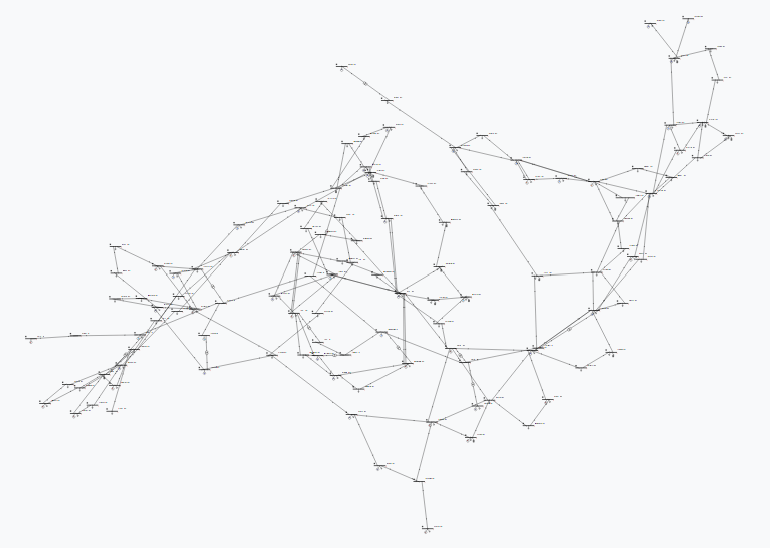
\includegraphics[width=0.8\textwidth]{chapter5pics/ieee118vanilla.png}
%     \caption{IEEE 118-bus system in GridCal.}
%     \label{fig:ieee118}
% \end{figure}
% \end{frame}

% \begin{frame}{Modified IEEE 118-bus (2)}
% \begin{figure}[H]
%     \centering
%     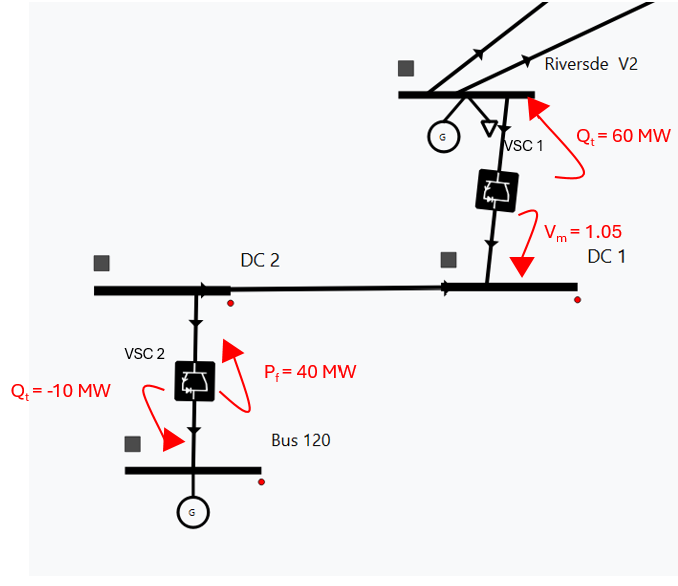
\includegraphics[width=0.6\textwidth]{chapter5pics/ieee118hvdc.png}
%     \caption{Control scheme of VSCs in IEEE 118-bus system.}
%     \label{fig:ieee118hvdc}
% \end{figure}
% \end{frame}


% \begin{frame}{Modified IEEE 118-bus (3)}
%     \begin{figure}[H]
%         \centering
%         \begin{tikzpicture}
%         \begin{semilogyaxis}[
%             title={\textbf{Raw Error Evolution}},
%             xlabel={Iterations},
%             ylabel={log(Error) (p.u.)},
%             width=\textwidth,
%             height=0.4\textwidth,  % Increased height
%             xmin=1, xmax=13,
%             ymin=1e-11, ymax=1e10,
%             log base 10 number format code/.code={\pgfmathprintnumber[fixed]{####1}},
%             max space between ticks=20,
%             legend pos=south west,
%             ymajorgrids=true,
%             grid style=dashed,
%             scaled ticks=false,
%             yticklabel style={/pgf/number format/sci},
%             legend style={font=\footnotesize},
%         ]

%         % Data for 'Raw Error'
%         \addplot[
%             color=blue,
%             mark=*,
%             mark options={solid}
%             ]
%             coordinates {
%                 (1, 92.73308863669693)
%                 (2, 55.85690495945452)
%                 (3, 9.8285672624759)
%                 (4, 0.5464519087140244)
%                 (5, 0.007224028507725633)
%                 (6, 0.00017727393030409627)
%                 (7, 2.706168691423566e-05)
%                 (8, 4.124082729088652e-06)
%                 (9, 6.28299001437238e-07)
%                 (10, 9.573791809325272e-08)
%                 (11, 3.371018117426239e-10)
%                 (12, 5.932321300861076e-11)
%                 (13, 0)
%             };
%             \addlegendentry{Generalised}
%             % Data for 'Classical Normalized Error'
%             \addplot[
%                 color=orange,
%                 mark=square*,
%                 mark options={solid}
%                 ]
%             coordinates {
%                 (1, 5.889388122682089)
%                 (2, 5280707.088151514)
%                 (3, 5280707.088151514)
%                 (4, 5280707.088151514)
%                 (5, 5280707.088151514)
%                 (6, 5280707.088151514)
%                 (7, 5280707.088151514)
%                 (8, 5280707.088151514)
%                 (9, 5280707.088151514)
%                 (10, 5280707.088151514)
%                 (11, 5280707.088151514)
%                 (12, 5280707.088151514)
%                 (13, 5280707.088151514)
%             };
%                 \addlegendentry{Classical}


            
%         \end{semilogyaxis}
%         \end{tikzpicture}
%         \caption{Raw Error Evolution for Modified IEEE 118-bus system.}
%     \end{figure}
% \end{frame}

% \subsection{Performance comparison}
% \begin{frame}{Runtimes (1)}

%     \begin{figure}[!htb]
%     \centering
%     \begin{tikzpicture}
%         \begin{axis}[
%             ybar,
%             title={\textbf{Runtime Comparison}},
%             ymin=0,
%             bar width=7pt,
%             width=\textwidth,
%             height=0.7\textheight,
%             enlarge x limits=0.25,
%             legend style={at={(0.5,-0.2)},
%             anchor=north,legend columns=-1},
%             ylabel={Runtime (ms)},
%             symbolic x coords={6-bus Grid, IEEE 14-bus, IEEE 118-bus},
%             xtick=data,
%             nodes near coords align={vertical},
%             x tick label style={anchor=north},
%             legend style={font=\footnotesize},
%             ymajorgrids,
%             grid style=dashed,
%         ]

%         % Generalised Power Flow
%         \addplot[fill=blue] coordinates {(6-bus Grid,404.08) (IEEE 14-bus,496.87) (IEEE 118-bus,740.60)};
        
%         % Classical Power Flow
%         \addplot[fill=orange] coordinates {(6-bus Grid,330.65) (IEEE 14-bus,444.47) (IEEE 118-bus,0)};

%         \legend{Generalised, Classical}
%         \end{axis}
%     \end{tikzpicture}
%     \caption{Runtime comparison for Generalised and Classical power flow.}
%     \label{fig:runtime}
%     \end{figure}

% \end{frame}

\begin{frame}{Runtimes (2)}

    % Table for Generalised and Classical Runtimes
    \begin{table}[H]
        \centering
        \caption{Runtime comparison (in milliseconds).}
        \begin{tabular}{|l|c|c|}
        \hline
        \textbf{Test Case} & \textbf{Generalised (ms)} & \textbf{Classical (ms)} \\ \hline
        6-bus Grid    & 404.08   & 330.65 \\ \hline
        IEEE 14-bus   & 496.87   & 444.47 \\ \hline
        IEEE 118-bus  & 740.60   & N/A    \\ \hline
        \end{tabular}
        \label{tab:runtime_comparison}
    \end{table}

    % Table for Runtime Breakdown
    \begin{table}[H]
        \centering
        \caption{Runtime breakdown for three test cases (in milliseconds).}
        \begin{tabular}{|l|c|c|c|}
        \hline
        \textbf{Test Case} & \textbf{Mismatch (ms)} & \textbf{Jacobian (ms)} & \textbf{Solve (ms)} \\ \hline
        6-bus Grid    & 1.7267   & 1.8666   & 2.2551    \\ \hline
        IEEE 14-bus   & 1.8940   & 2.2084   & 2.9206    \\ \hline
        IEEE 118-bus  & 3.7404   & 6.1091   & 5.5986    \\ \hline
        \end{tabular}
        \label{tab:runtime_breakdown}
    \end{table}

\end{frame}

